\documentclass[letterpaper, 10 pt, conference]{ieeeconf}  % Comment this line out

\IEEEoverridecommandlockouts                              % This command is only
                                                          % needed if you want to
                                                          % use the \thanks command
\overrideIEEEmargins

\usepackage{amsmath}    % need for subequations
\usepackage{graphicx}   % need for figures
\usepackage[font=footnotesize,labelfont=footnotesize]{caption}
\usepackage{verbatim}   % useful for program listings
\usepackage{color}      % use if color is used in text
\usepackage{subfigure}  % use for side-by-side figures
\usepackage{subcaption}
\usepackage{hyperref} % use for hypertext links, including those to external documents and URLs
\usepackage{multirow}
\usepackage{rotating}
\usepackage{array}
\usepackage{xspace}
\usepackage{indentfirst}
\usepackage{amssymb}
\usepackage{float}
\usepackage{algorithm}
\usepackage{algorithmic}
\usepackage{comment}
\usepackage{sidecap}
\usepackage{booktabs}

\title{Mobile Robots in Polygons: a Combinatorial Data Structure for
Navigation, Localization, and Coverage}

\author{Alexandra Q. Nilles, Yingying Ren% <-this % stops a space
%\thanks{This work was partially supported by National Science Foundation (award numbers CMMI-1100579 and IIS-1302393).}
}

\begin{document}


\maketitle

%%%%%%%%%%%%%%%%%%%%%%%%%%%%%%%%%%%%%%%%%%%%%%%%%%%%%%%%%%%%%%%%%%%%%%%%%%%%%%%%
%\begin{abstract}
%
%\end{abstract}

{\small
\begin{center}
\begin{quotation}
``Geometry is not true, it is advantageous." \\
\hfill    --- Henri Poincar\'e
\end{quotation}
\end{center}
}

%%%%%%%%%%%%%%%%%%%%%%%%%%%%%%%%%%%%%%%%%
\section{Introduction} 
% There has been rising interests in minimum sensing robots in recent years as swarm robots become more and more popular. 
In this paper, we consider simple robots with "bouncing" behaviors: robots which travel in straight lines in the plane, until encountering an environment boundary, at which point they rotate in place and set off again. A growing line of work is considering the computational power of individual bouncing strategies and their applications to robotic tasks and applications in biological contexts \cite{erickson2013toward}, \cite{microorg}, \cite{alam2017minimalist}. 

We introduce a combinatorial, visibility-based data structure to organize and compare these bouncing strategies in simple polygonal environments. The overall idea is to discretize the environment boundary using visibility information, creating equivalence classes (segments along the boundary) where the robot has a similar set of choices from any point in the segment. We then construct a graph representation of this environment where nodes are segments of the boundary, and edges are transitions between segments (with associated control strategies). We then extend previous results on the dynamics of composed transitions \cite{nilles2017periodic}, which give convenient guarantees on the stability of cycles and contraction of robot state uncertainty. Finally, we demonstrate how to formulate many common mobile robotic tasks as queries to this data structure.


\subsection{Robot Motion Model}\label{subsec:bounce_strategy}

A polygon is in general position if no $3$ vertices lie on the same line. For the rest of this paper, we assume all polygons are in general position. All index arithmetic is $\mod n$ throughout the paper.

A \emph{bouncing strategy} describes the robot's configuration change when it encounters the boundary of a polygon. We will only consider the bounce occurred inside an open edge of the polygon: the robot's behavior is undefined at a vertex of the polygon. Each bouncing strategy has a characterization function for $\vec{m}$ over parameters $\vec{n}$ and $\vec{l}$, where $\vec{n}$ is the unit vector for the normal of the bounce-off wall, $\vec{l}$ is the unit vector for the incoming direction, and $\vec{m}$ is the unit vector for the outgoing direction.
\begin{itemize}
    \item Specular Bounce (Billiard): $\vec{m} = f(\vec{l}, \vec{n})$, where \begin{eqnarray*}
    f(\vec{l}, \vec{n}) = \vec{l} - 2(\vec{l}\cdot \vec{n})\vec{n}
    \end{eqnarray*}
    (``$\cdot$'' is the dot product operation between two vectors), which is equivalent to $(\vec{l}+\vec{m}) \cdot \vec{n} = 0$. This bouncing behavior is elastic and follows the most natural law: the incoming angle equals the outgoing angle \cite{geometry_billards}.
    \item Fixed Angle Bounce: $\vec{m} = f(\vec{n}, \theta)$, where $\theta$ is a constant in $[-\frac{\pi}{2}, \frac{\pi}{2}]$, and \begin{eqnarray*}f(\vec{n}, \theta) = 
    \begin{bmatrix} 
    \cos(\theta) & \sin(\theta)\\
    -\sin(\theta) & \cos(\theta)\\
    \end{bmatrix}\vec{n}.\end{eqnarray*} In other words, the robot always bounces off the wall at a fix angle with respect to the normal.
    \item Monotonic Fixed Angle Bounce: $\vec{m} = f(\vec{l}, \vec{n}, \theta)$, where $\theta$ is a constant in $(0, \frac{\pi}{2})$. Let $s = det(\begin{bmatrix} 
    \vec{l}.x & \vec{l}.y\\
    \vec{n}.x & \vec{n}.y\\
    \end{bmatrix})$, and $\theta' = \frac{s}{|s|}\theta$ ($|s|$ denote the absolute value of $s$; the behavior for $|s| = 0$ is undefined). Then \begin{eqnarray*}f(\vec{l}, \vec{n}, \theta) = 
    \begin{bmatrix} 
    \cos(\theta') & \sin(\theta')\\
    -\sin(\theta') & \cos(\theta')\\
    \end{bmatrix}\vec{n}.\end{eqnarray*} This bouncing strategy is very similar to the Fixed Angle Bounce except for the monotonic restriction that the robot's incoming path and outgoing path have to be on the opposite sides of the normal.
    
    \item Relative Angle Bounce: $\vec{m} = f(\vec{l}, \beta)$, where $\beta$ is a constant in $[0, 2\pi)$, and \begin{eqnarray*}f(\vec{l}, \beta) = \begin{bmatrix}
    \cos(\beta) & -\sin(\beta)\\
    \sin(\beta) & \cos(\beta)\\
    \end{bmatrix}\vec{l}.
    \end{eqnarray*} The robot will rotate a fixed angle $\beta$ counter-clockwise when encountering the wall. It is possible that this rotation will cause the heading of the robot to still be facing into the wall, in which case this model usually has the robot perform the rotation again until it's heading points into the free space.
\end{itemize}

% fixed vs. monotonic fixed vs. relative vs. specular

% parameterization for monotonic bounces: alpha + beta + gamma = pi

% all bounces are some function of incoming angle and wall normal

\subsection{Related Work}

In \cite{microorg}, the authors show that a \textit{Chlamydomonas reinhardtii} cell would bounce off a surface with a monotonic fixed angle bounce. This line of work characterizes periodic and chaotic trajectories in regular polygons, planar curves, and other environments. They analyze dynamics of fixed bounce angles, without a focus on control.

\cite{lewis2013planning} partially solved the navigation task with a very similar robot
model. Their robot moves in straight lines until encountering an environment
boundary, at which point it is able to rotate in place, with some nondeterministic but
bounded error. They then generate a strategy as a sequence of bounce angles which can navigate the robot between given start and end locations in a known environment. Their approach only allows "safe actions," which place
the entire forward projected state of the robot within a single
linear segment of the polygonal environment. They then solve the navigation task by
planning in a graph where each node is a point or segment
location of the robot, and edges are safe actions. However, this algorithm is
not complete, due to the restriction on safe actions -
sometimes the uncertainty of the actuators make it impossible to create a
strategy which only uses safe actions. Additionally, it requires hand-crafted local planners for navigating long hallways, due to the way the environment segmentation is done. At most, their graph search has $O(n^4)$ nodes, which is the same complexity as our proposed data structure, but our method can also achieve navigation without hand-crafted local planners due to the visibility-based decomposition of the environment boundary.

In \cite{alam2017minimalist} and \cite{alam2018space}, the authors describe navigation, coverage, and localization algorithms for a robot with a clock and contact sensor that is capable of performing relative angle bounces. Their approach uses a discretization of the robot configuration space and actuation space, then searches the discretized dynamical system for limit cycles. The algorithm is complete and correct up to discretization error - periodic trajectories may exist which require bounce angles not allowed by the discretization. Our work is very similar in spirit to this approach, however, we use a more natural discretization induced by the environment geometry and consider all possible bounce strategies in our combinatorial representation. Our representation may be reduced to one which can be used to solve the same problems as this work, by applying constraints on the types of bounces allowed.



\section{Combinatorial Visibility Data Structures}

We will provide an overview of some data structures related to visibility in polygons, some of which we are using directly, and some of which provided inspiration for this work.

\subsection{Visibility Graphs}


Let $P$ be a polygon in $\mathbb{R}^2$ with $n$ vertices $(v_0, v_1, \ldots, v_{n-1})$. An edge of $P$ is represented as $e_i = v_iv_{i+1}$. 

The \textit{vertex visibility graph} $G_V(P) = (V, E)$ has $V = \{v_0, v_1, \ldots, v_{n-1}\}$ and $v_iv_j\in E$ if and only if the segment connecting $v_i$ and $v_j$ is completely contained in the interior of $P$. We call $v_i, v_j$ visible to each other if $v_iv_j\in E$. By definition, the vertex visibility graph for a convex polygon with $n$ vertices is a $n-$clique. Fig~\ref{fig:vvg} shows the visibility graph for a non-convex polygon.
\begin{figure}
    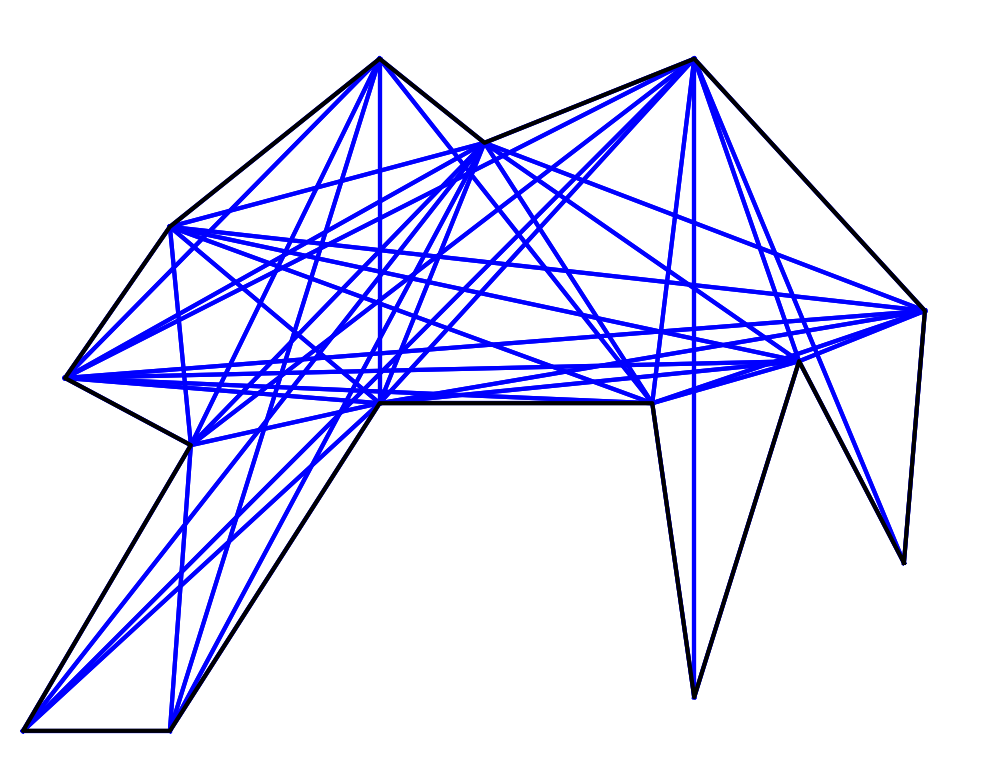
\includegraphics[width=0.8\linewidth]{images/viz_graph.png}
    \centering
    \caption{The vertex visibility graph}\label{fig:vvg}
    \centering
\end{figure}

We can also define the \textit{vertex-edge visibility graph} for a polygon. Using the definition in \cite{rourke_viz}, the \textit{vertex-edge visibility graph} for $P$, $G_E(P) = (V, E)$, is a bipartite graph where $V = \{\text{all vertices and edges in $P$}\}$ and $v_ie_j\in E$ if and only if $v_i$ can see the interior of $e_j$, i.e., $\exists$ point $q$ on the open edge $e_j$ such that $v_i$ and $q$ are visible. \cite{rourke_viz} established that the vertex-edge visibility graph is equivalent to the edge-edge visibility graph. Fig~\ref{fig:veg} shows an example for vertex-edge visibility graph.
\begin{figure}
\centering
\subfigure[]{
\centering
  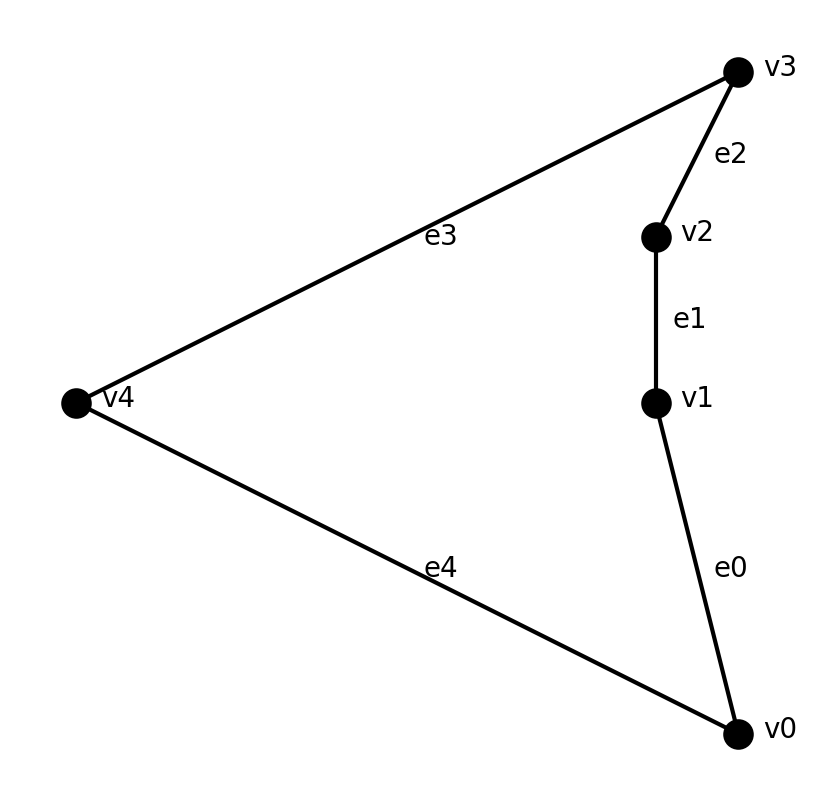
\includegraphics[width=0.6\linewidth]{images/concave_pent.png}
  \centering
  \label{fig:c_p}
}
\subfigure[]{
  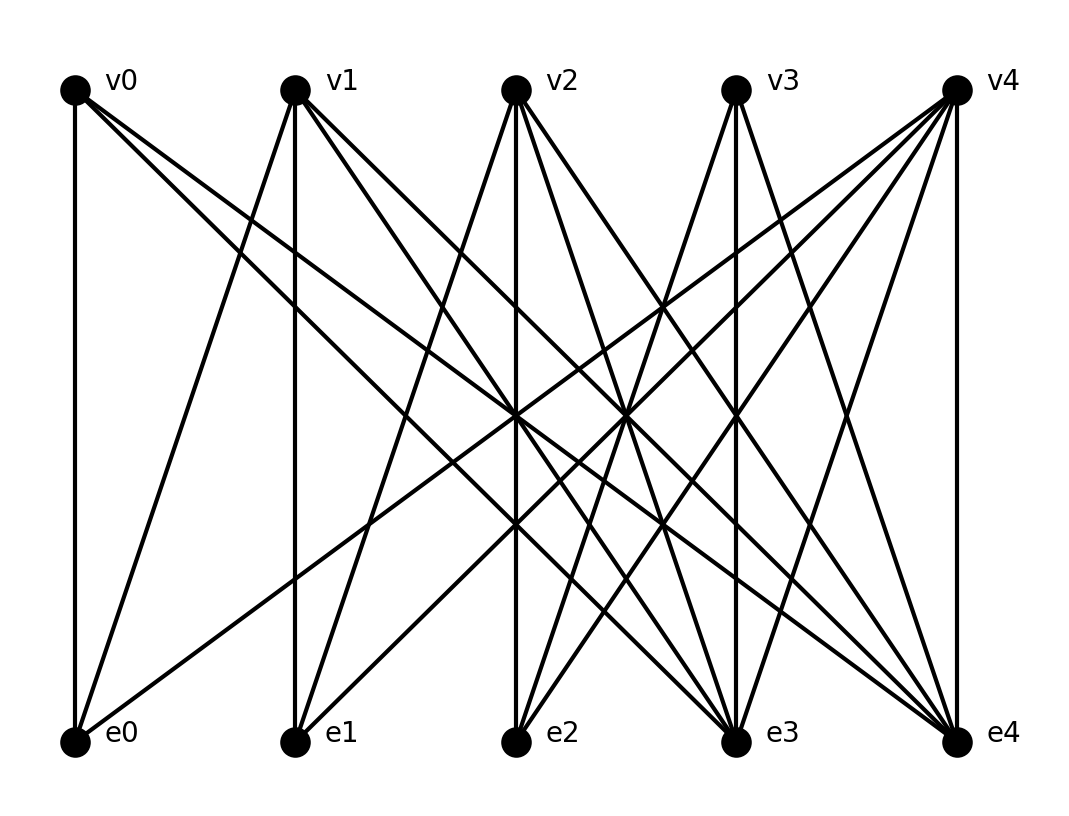
\includegraphics[width=0.8\linewidth]{images/viz_edge_graph.png}
  \centering
}
\caption{The vertex-edge visibility graph for the polygon in Fig~\ref{fig:c_p}}\label{fig:veg}

\end{figure}



\subsection{Partial local sequence}

The partial local sequence for a vertex $v_0$ in polygon $P$ contains new vertices created by the intersection of a ray, $r$, from each of the other vertices in $P$ to $v_0$ and the boundary of $P$ if $r$ exits $P$ at an edge of $P$. For example, in Fig~\ref{fig:pls}, the vertices in the partial local sequence of $v_0$ but not in the original polygon is annotated with blue dots.
\begin{figure}
    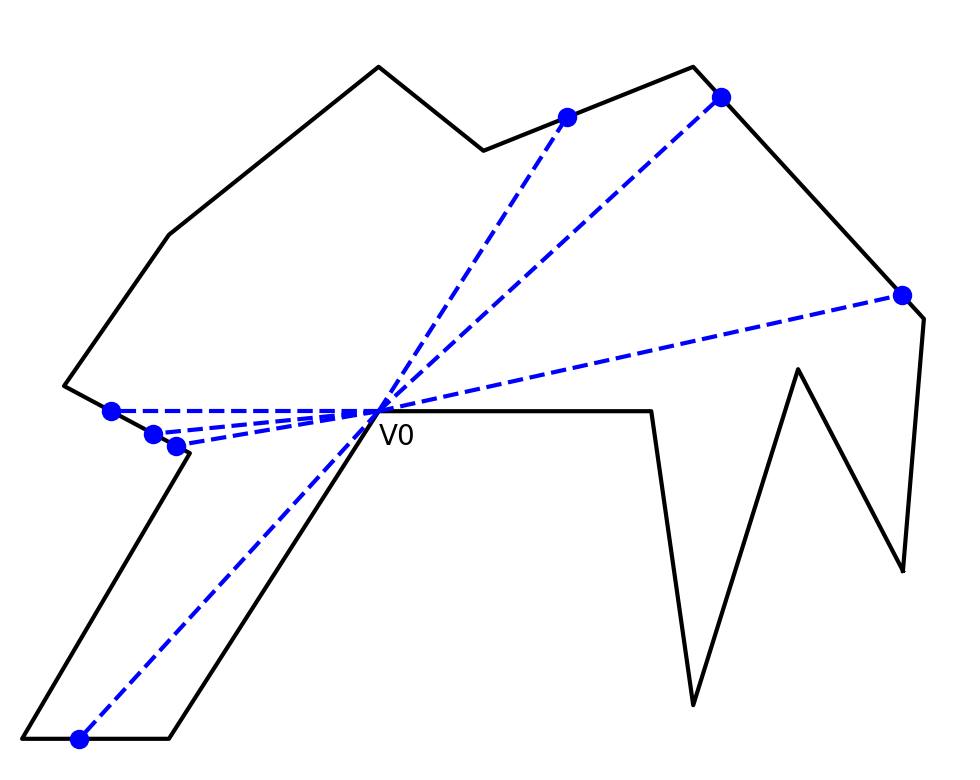
\includegraphics[width=0.8\linewidth]{images/partial_local_sequence.png}
    \centering
    \caption{Partial local sequence for $v_0$}\label{fig:pls}
    \centering
\end{figure}
The partial local sequences for vertices in a polygon is helpful for defining the equivalent class of edge visibility.



\subsection{Link diagram}

The link distance between two vertices in a polygon is the minimum number of line segments inside the polygon connecting the two vertices. The link distance between visible vertices is $1$. In Fig~\ref{fig:link_dis}, the link distance between $v_1$ and $v_2$ is 3.

The link diagram, as introduced in \cite{tan_sweep}, displays the link distance between any two points on the boundary of the polygon. \textcolor{red}{Do we need to create our own picture for link diagram here} The link diagram is our main motivation for creating a visibility diagram augmented with bouncing information.
\begin{figure}
    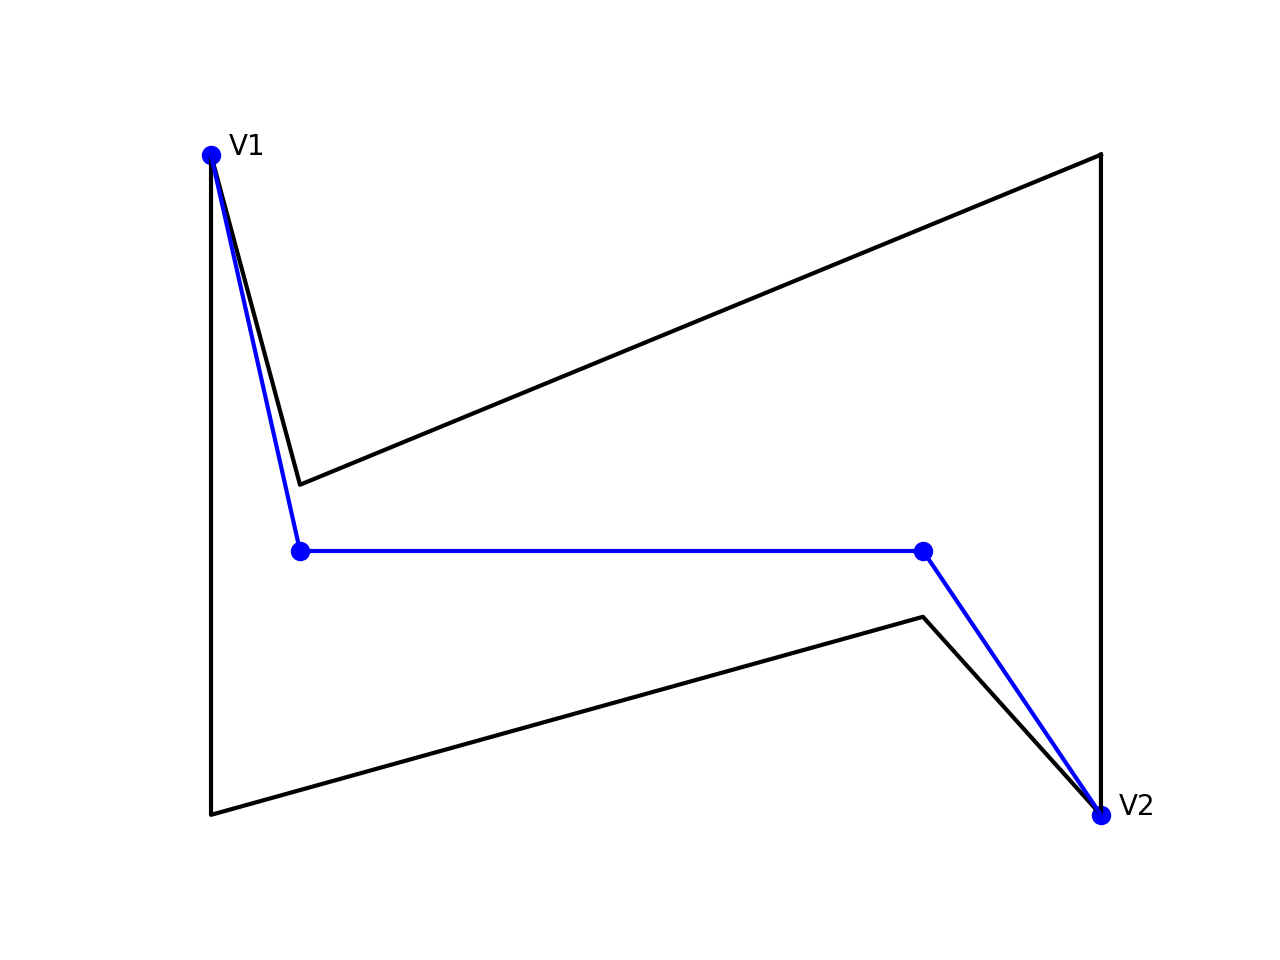
\includegraphics[width=0.6\linewidth]{images/link_distance.png}
    \centering
    \caption{The link distance between $v_1$ and $v_2$ is 3, as shown by the three blue line segments connecting the two vertices.}\label{fig:link_dis}
    \centering
\end{figure}

\section{Bounce Visibility Diagram}
We will now define the central structure for this paper, the \textit{Bounce Visibility Diagram} for polygon $P$. We will first insert all new vertices appeared in the partial local sequence for all vertices into the polygon $P$ to get the new polygon $P'$ with $m$ vertices. We intentionally create degeneracies here for reasons that will be revealed later.

The $x-$axis of the diagram parameterizes the boundary of the new polygon, denoted as $\partial P'$, in counterclockwise order to  $[0, m+1)$. We map every point in $\partial P'$ to a point in $[0, m+1)$; vertex $v_i$ on $\partial P'$ will map to $x = i$; all points in the open edge $v_iv_{i+1}$ will uniformly map to $(i, i+1)$. Let $f: [0, m+1)\mapsto \partial P'$ denote this parameterization. 

The vertical axis $\theta$ of the diagram has range $[0, \pi]$, representing all the possible angles the robot can bounce to. At angle $0$, the robot can bounce to the vertex in the front when it travels counterclockwise on $\partial P'$. Let the robot's ``forward direction'' be the direction of the edge that the robot is on in counterclockwise order. 

For each vertex $v_i$, we can define a function $B_i: [0, n) \mapsto [0, \pi]$ for the angle between the robot's forward direction and its direction to vertex  $v_i$ when the robot stands at $f(x)\in \partial P'$. $B_i$ are piecewise continuous functions; the discontinuities occur when $x$ is an integer, or, in other words, at the vertices of $\partial P'$. The original vertices in $P$ mark discontinuities because the angle reference frame for the robot changes when it moves to a new edge; the new vertices in $P'$ mark discontinuities because the robot has different vertex visibility view around those vertices, which motivates us to compute the partial local sequences in the first place. Fig~\ref{fig:bvd} shows an example of the bounce visibility diagram. 
\begin{figure}
\centering
\subfigure[]{
\centering
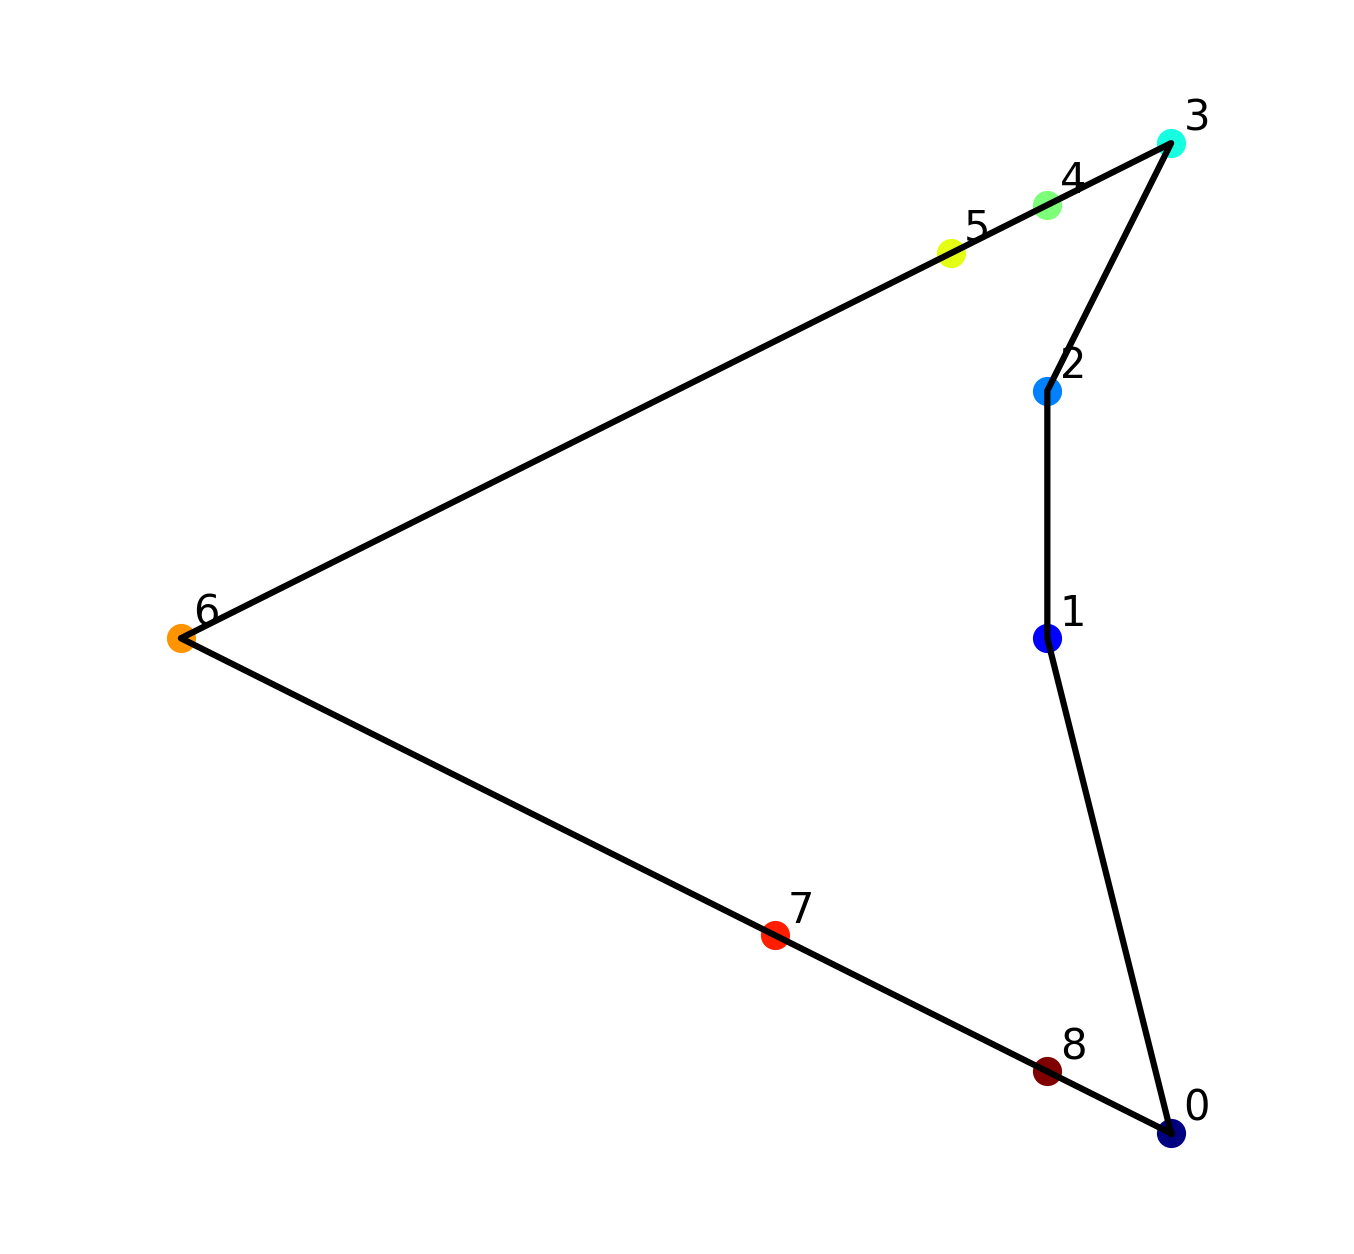
\includegraphics[width=0.7\linewidth]{images/color_pent.png}
\label{fig:color_pent}
}
\subfigure[]{
\centering
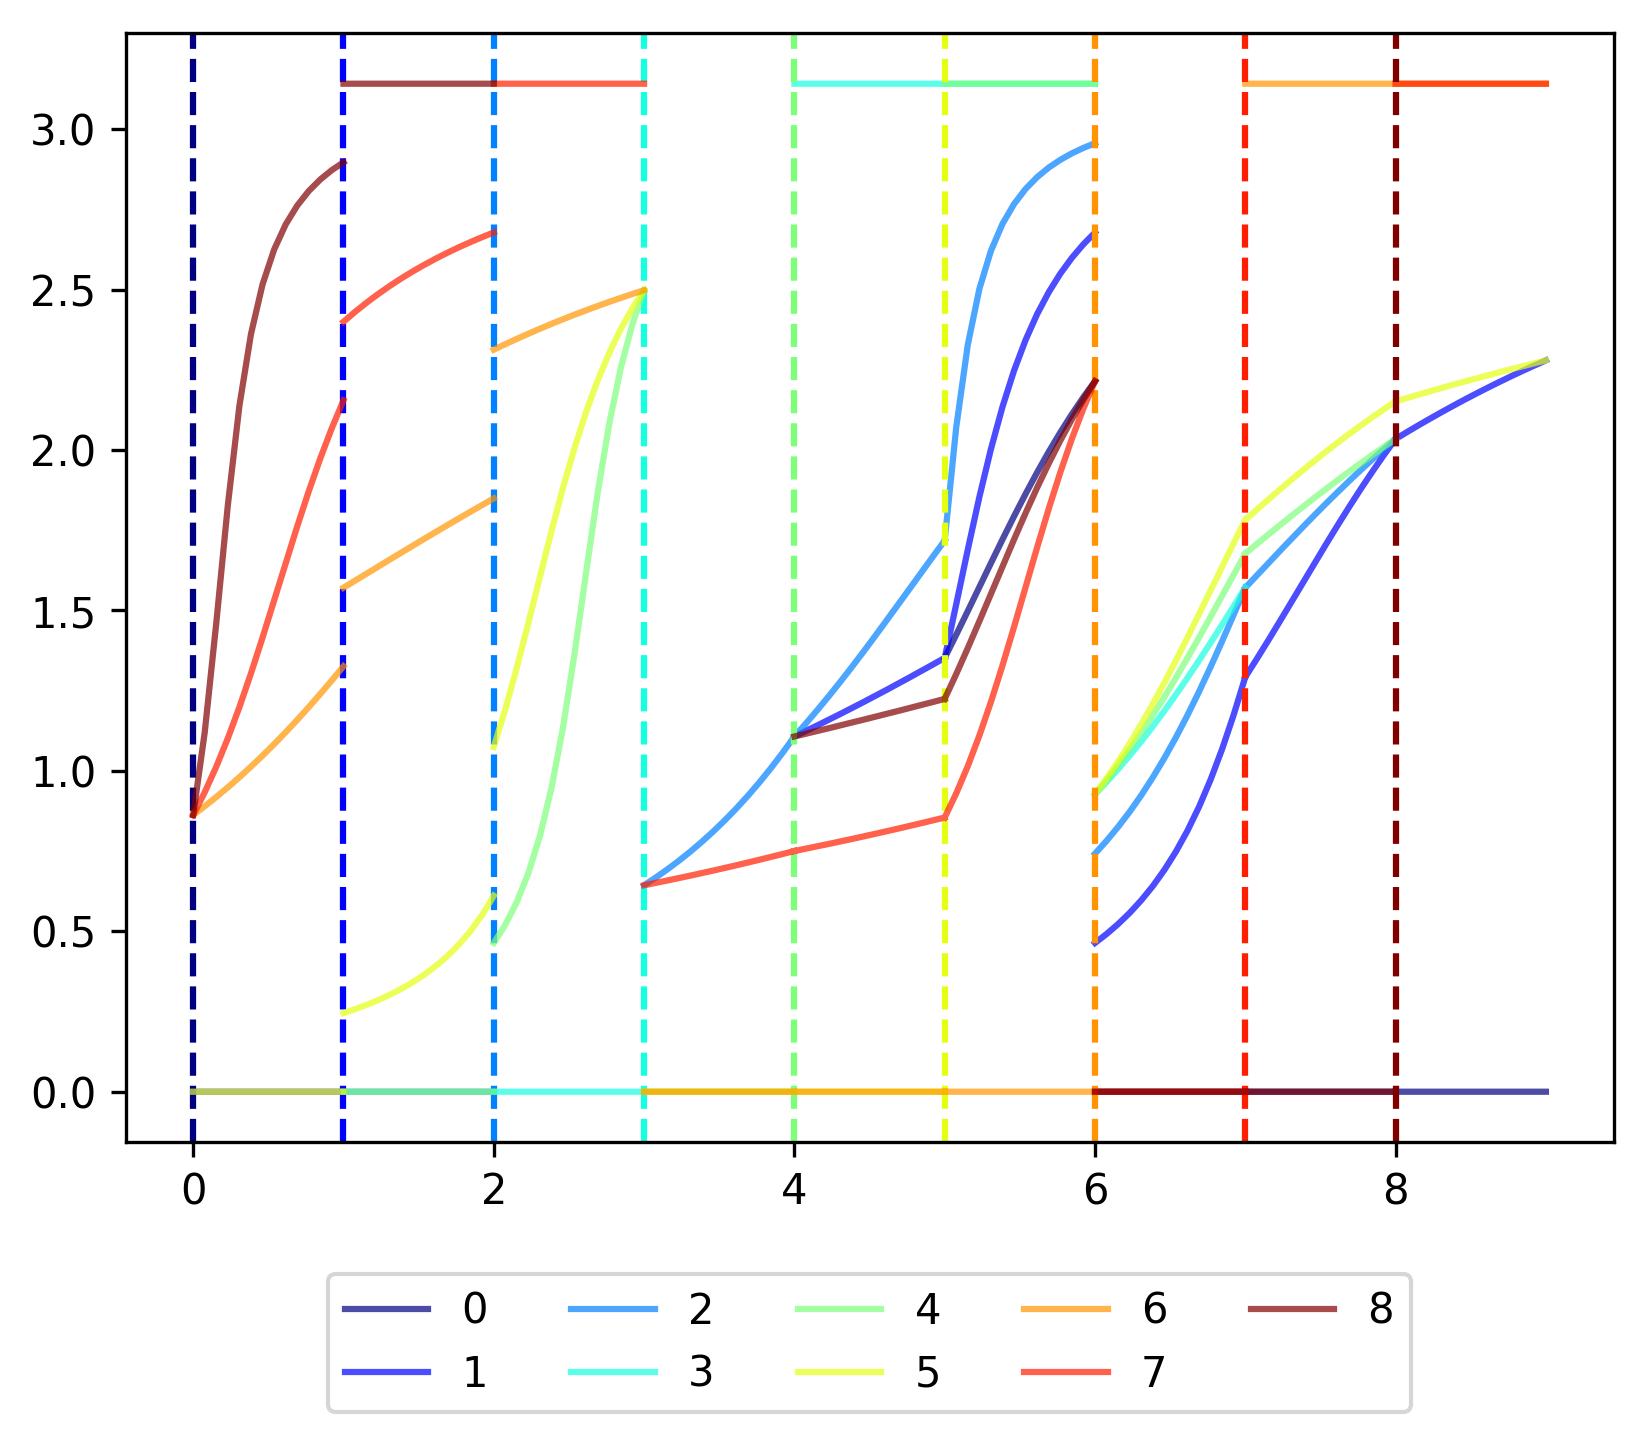
\includegraphics[width=0.8\linewidth]{images/bvd.png}
}
\caption{The bounce visibility diagram for the polygon shown in Fig~\ref{fig:color_pent}. }
\label{fig:bvd}

\end{figure}

\subsection{Properties of BVD}
The bounce visibility diagram can generate the vertex visibility graph by construction. In \cite{rourke_viz}, the authors point out that if the robot can see a vertex, then it can see the two edges connected to that vertex if the vertex is convex; otherwise, it can see one of the edges connected to that vertex. As the robot moves along an edge in the original $P$, its vertex visibility view changes, as shown for $x\in (3, 6)$ in Fig~\ref{fig:bvd}. The region between curve 2 (blue) and curve 7 (red) is subdivided as the $x$ increases, which corresponds to the robot has increasing knowledge about things behind the gap between vertices $v_2$ and $v_7$ as it moves along the edge $v_3v_6$: the appearance of gap between vertices $v_1$ and $v_8$, and the appearance of vertex $v_0$. For $x\in (6, 9]$, the diagram shows a reverse process of disappearance of gaps. By incorporating the information of the appearance and disappearance of gaps, we can also generate the vertex-edge visibility graph from the bounce visibility diagram. 
% (\textcolor{red}{I don't have proof yet but I think there are enough info to do that. We can also shift this part about gap navigation into later sections.})

Circular symmetries in a polygon can be reflected in the periodic structure of the corresponding BVD, as shown in Fig~\ref{fig:regular_pent_bvd}.

\begin{figure}
% \makebox[\linewidth][c]{%
\subfigure[]{
\centering
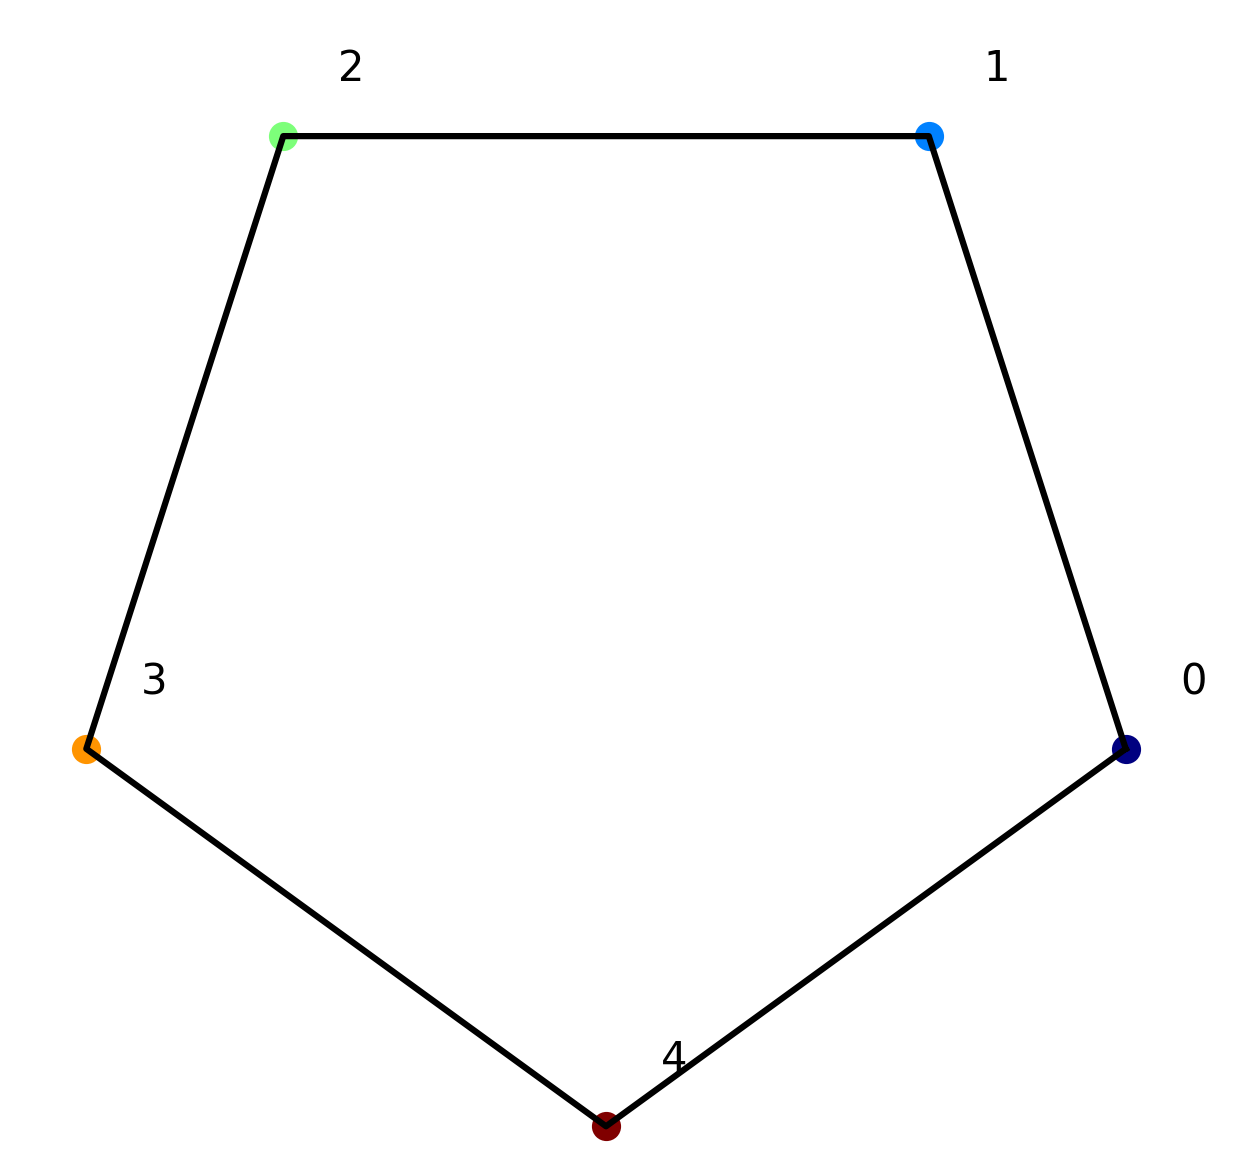
\includegraphics[width=0.5\linewidth]{images/regular_pent.png}
}
\centering
\subfigure[]{
\centering
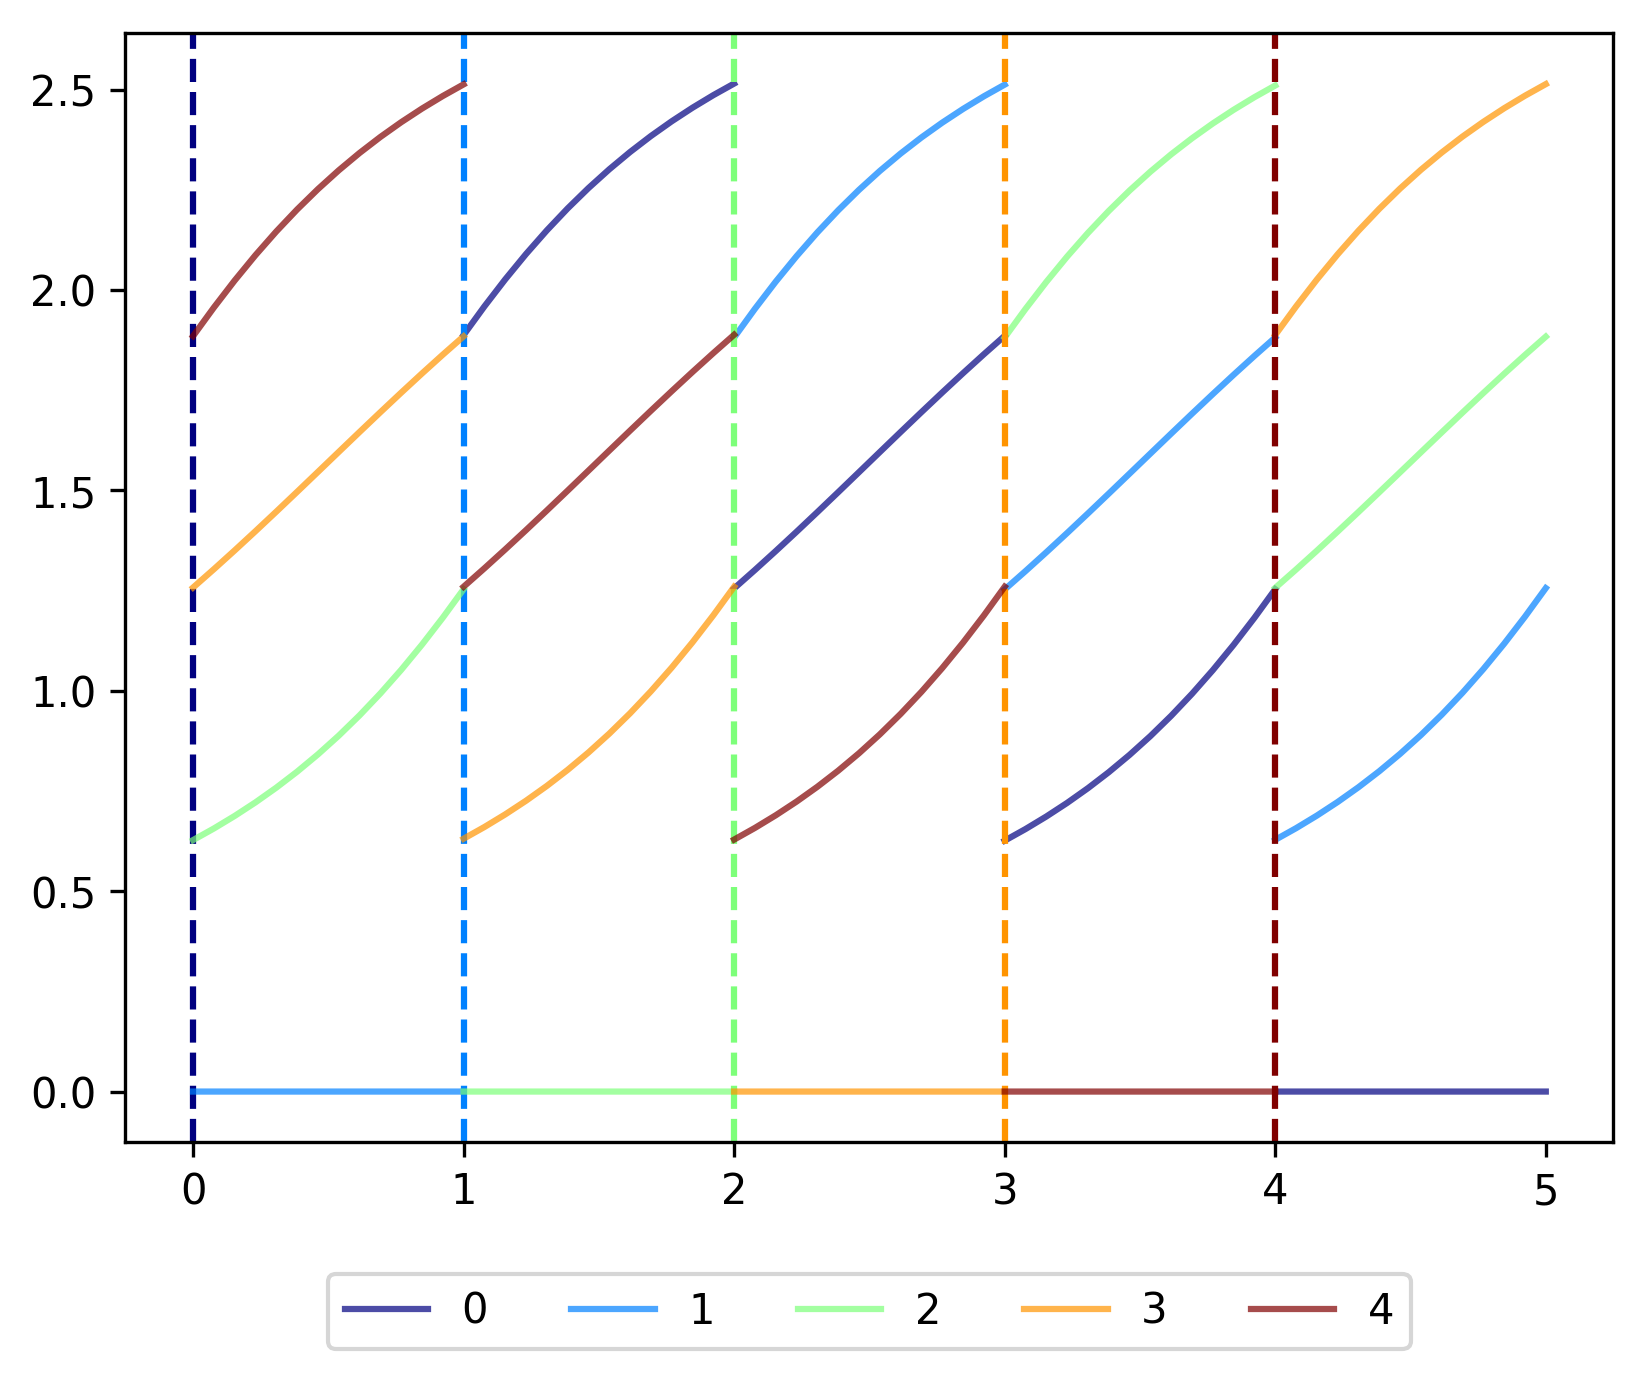
\includegraphics[width=0.8\linewidth]{images/regular_pent_bvd.png}
}
\centering
% }\\
\caption{The bounce visibility diagram for the regular pentagon. }
\label{fig:regular_pent_bvd}
\end{figure}
We can easily extract information for the fixed angle bouncing strategy mentioned in section~\ref{subsec:bounce_strategy} by overlaying an horizontal line $\theta = \theta_0$ onto the BVD, where $\theta_0$ is the angle chosen by the bouncing strategy. In Fig~\ref{fig:limit_cycle_bvd}, one of the possible limit cycle with fixed angle $\theta = 0.6$ for the concave quadrilateral is shown in Fig~\ref{fig:limit_cycle}; the bounce visibility diagram for this polygon is shown in Fig~\ref{fig:concave_quad_bvd} with the horizontal line $\theta = \theta_0$, where $\theta_0 = \frac{\pi}{2}-0.6$ (we need to convert the angle from w.r.t the normal of the wall to w.r.t the forward direction of the robot). The horizontal line cut through different regions of the diagram, representing the possible edges that the robot can bounce to at different points on the boundary with bounce angle $\theta_0$. For example, at edge $v_5v_0$, the robot can bounce to edge $v_0v_1$ and $v_1v_2$. We can create a graph for $\theta = \theta_0$, whose nodes are edges in $P'$ and two nodes are connected by a directed edge if the robot can bounce from one edge to another at $\theta_0$, as shown in Fig~\ref{fig:limit_cycle_diagram}. It is more stable for the robot to bounce to some edges than others. In the diagram (Fig~\ref{fig:concave_quad_bvd}), the line $\theta = \theta_0$ cuts through four different regions for $x \in (2, 3)$, but the sections for $v_4v_5$ and $v_0v_5$ are much larger than those for $v_0v_1$ and $v_1v_2$. So we know it is more likely and more stable for the robot to bounce to edge $v_4v_5$ and $v_0v_5$. We marked the edge with unstable bounce in the graph with $\omega$ in Fig~\ref{fig:limit_cycle_diagram}. The limit cycle shown in Fig~\ref{fig:limit_cycle} corresponds to the cycle $v_0v_1\rightarrow v_3v_4\rightarrow v_4v_5 \rightarrow v_1v_2 \rightarrow v_2v_3 \rightarrow v_0v_5 \rightarrow v_0v_1$ in Fig~\ref{fig:limit_cycle_diagram}.
(\textcolor{red}{do we talk about this here or later in the task})
\begin{figure}
\centering
\makebox[\linewidth][c]{%
\subfigure[]{
\centering
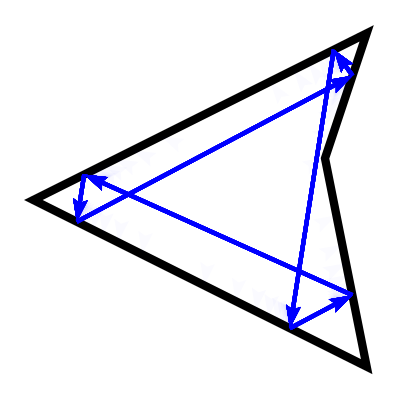
\includegraphics[width=0.45\linewidth]{images/limit_cycle_concave_quad.png}
\label{fig:limit_cycle}
}
\subfigure[]{
\centering
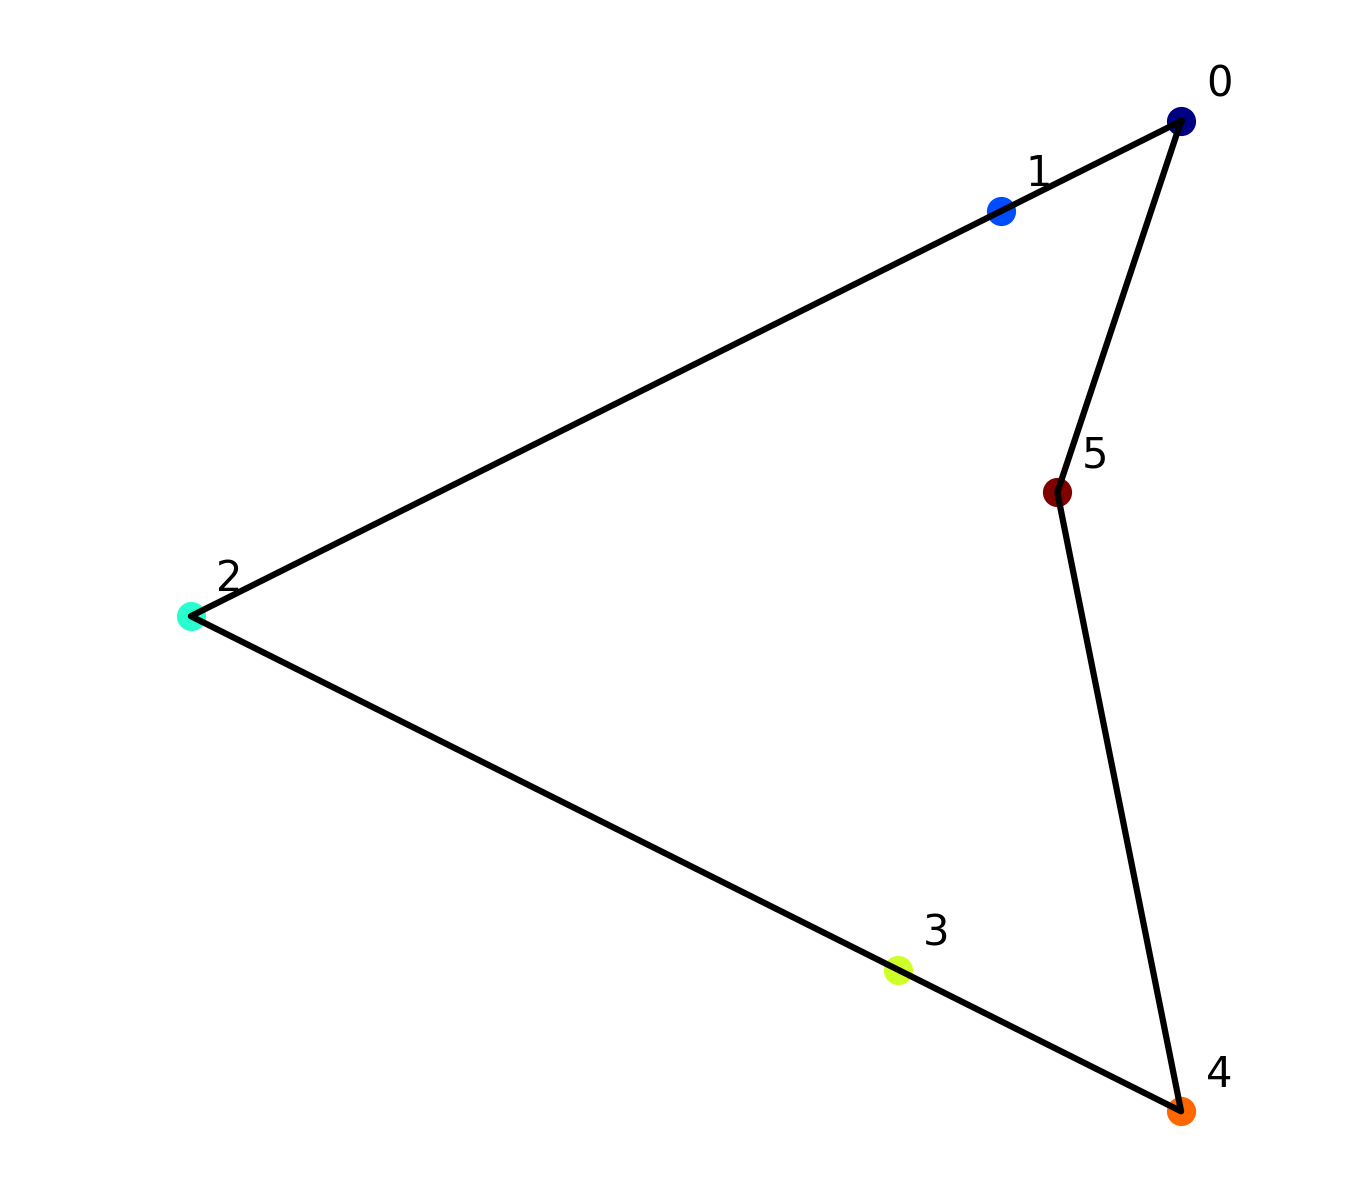
\includegraphics[width=0.52\linewidth]{images/concave_quad.png}
}
\label{fig:color_concave_quad}
}\\
\subfigure[]{
\centering
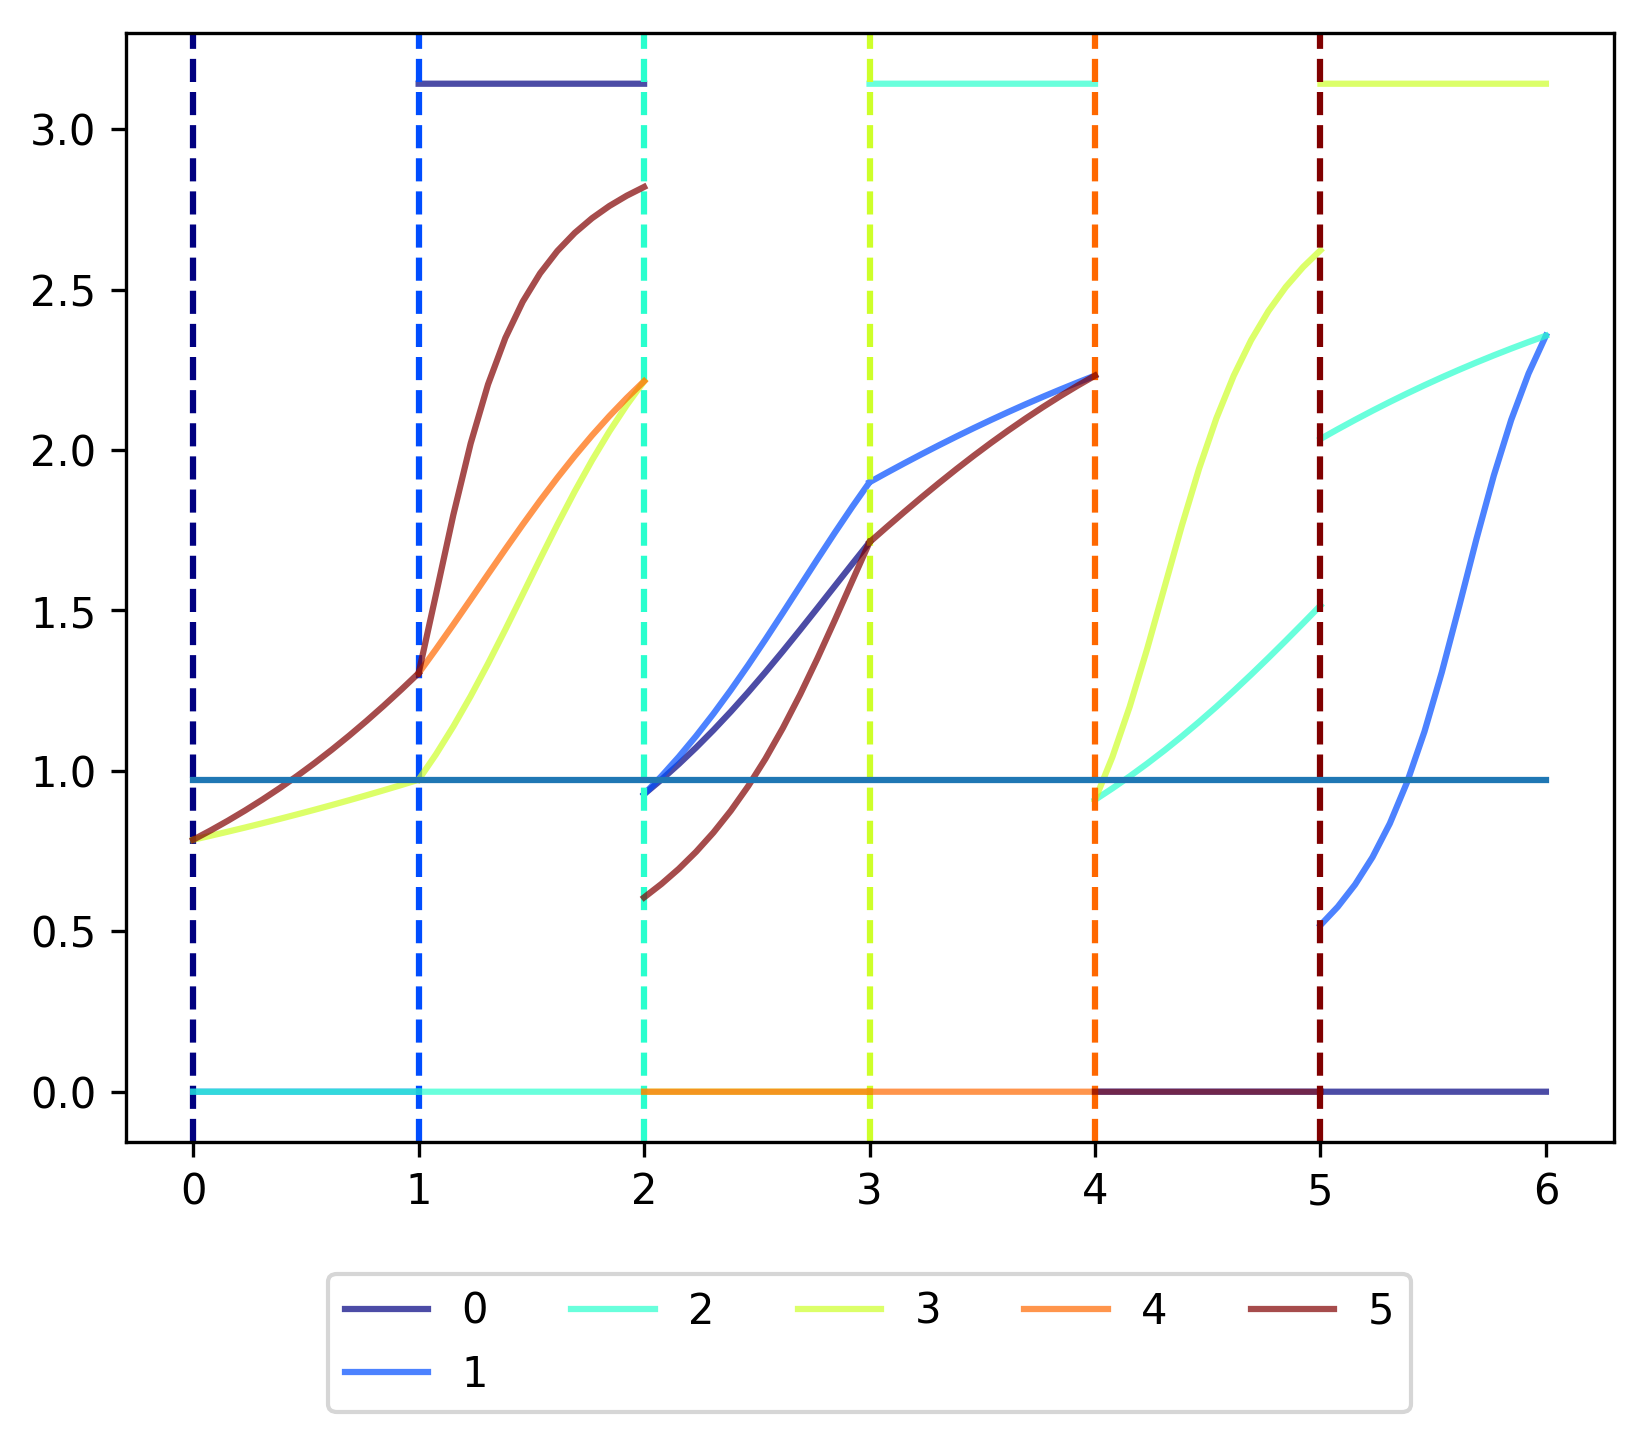
\includegraphics[width=0.8\linewidth]{images/limit_cycle_bvd.png}
\label{fig:concave_quad_bvd}
}
\subfigure[]{
\centering
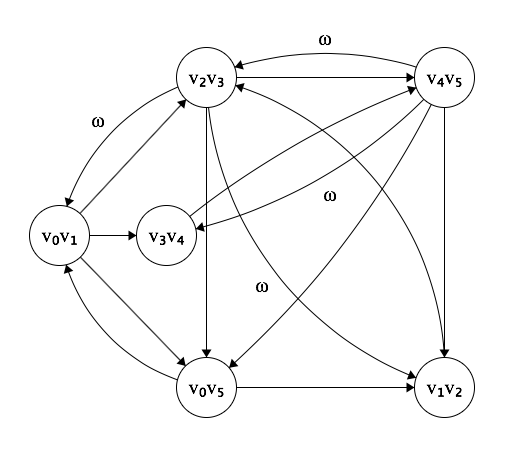
\includegraphics[width=0.8\linewidth]{images/limit_cycle_graph.png}
\label{fig:limit_cycle_diagram}
}
\caption{The bounce visibility diagram with limit cycle information}
\label{fig:limit_cycle_bvd}
\end{figure}

\subsection{Combinatorial Complexity of BVD}

To consider the size of the bounce visibility diagram for an input polygon $P$ with $n$ vertices, we let $r$ be the number of reflex vertices in the polygon, and $m$ be the average number of visible vertices to a vertex in $P'$. For a convex vertex, its partial local sequence will not have new vertex that is not in $P$, while for a reflex vertex, we can have $O(n)$ new vertices. We can have as many as half of the vertices to be reflex, so $r = O(n)$; each of the reflex vertices can produce $O(n)$ new vertices in its partial local sequence, so the size of $P'$ is $O(n^2)$. It is possible for a vertex in $P'$ to see all other vertex, so, in the worse case, $m = O(n^2)$. Therefore, the complexity of the bounce visibility diagram is $O(n\cdot r\cdot m) = O(n^4)$. 

We might hope that if $r$ is large, then not all of the reflex vertices will produce a large number of new vertices, or that if there are many new vertices, then the new vertices will not have good visibility in $P'$ since most of them will be inserted into a corner of the polygon, and then we can bound the complexity of the BVD. Unfortunately, the number of reflex vertices, the new vertices produced in their partial local sequence, and the new vertices' visibility can be large at the same time. We will present a family of input polygons with BVD of $\Theta(n^4)$ complexity as follows. 
\begin{figure}
\hspace{-40px}
\centering
\makebox[\linewidth][c]{%
\hspace{30px}
\subfigure[]{
\centering
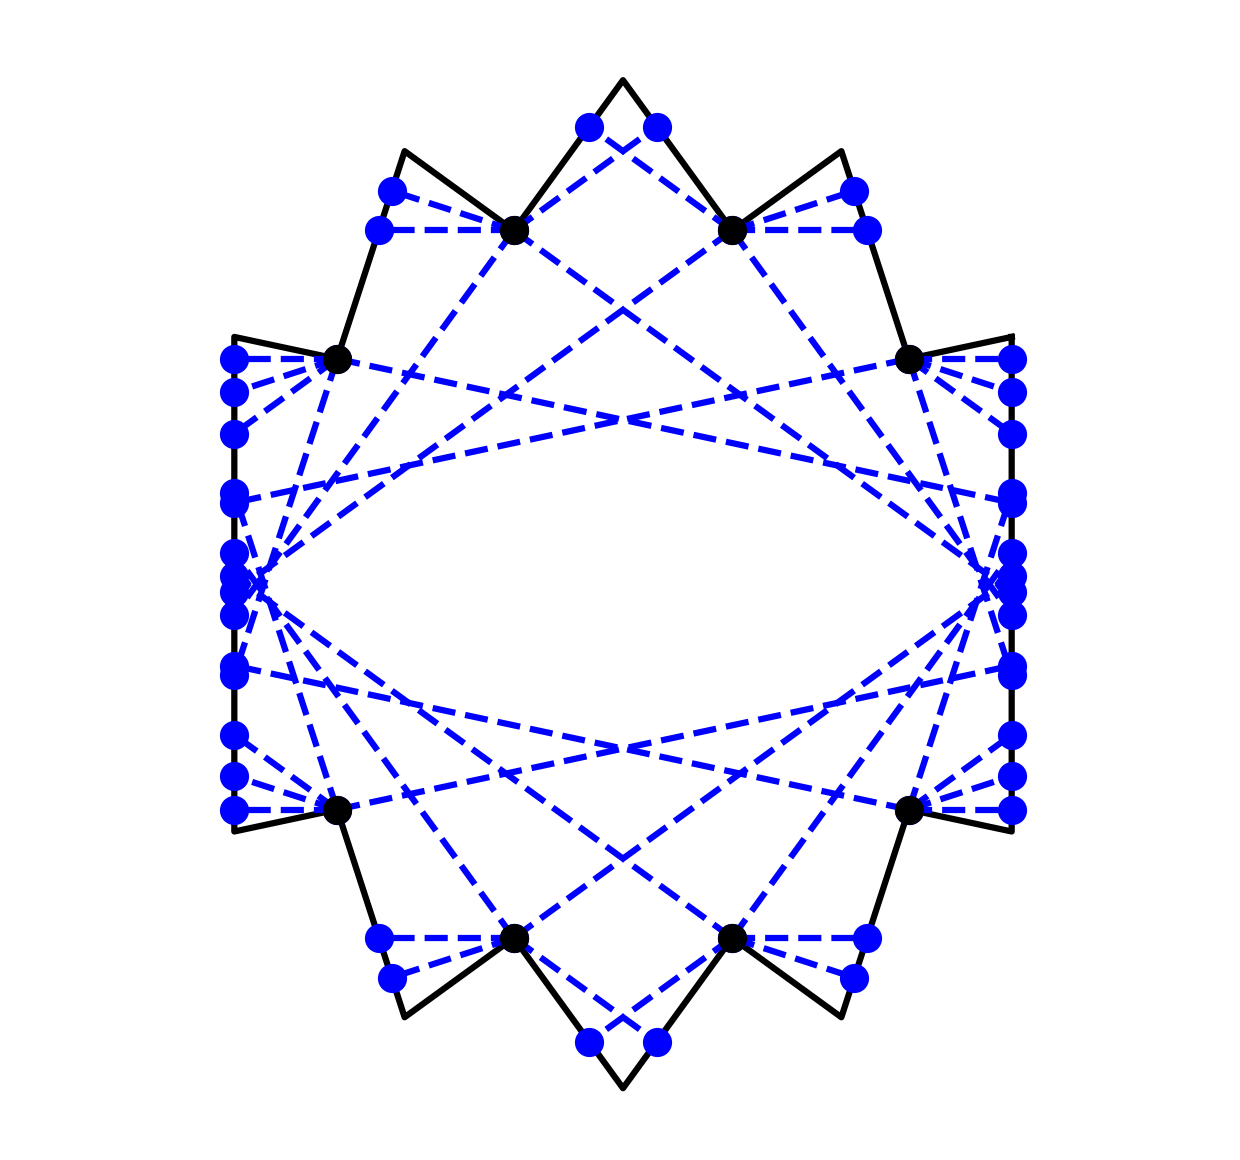
\includegraphics[width=0.7\linewidth]{images/chestnut_5.png}
\label{fig:t4}
}
\hspace{-40px}

\subfigure[]{
\centering
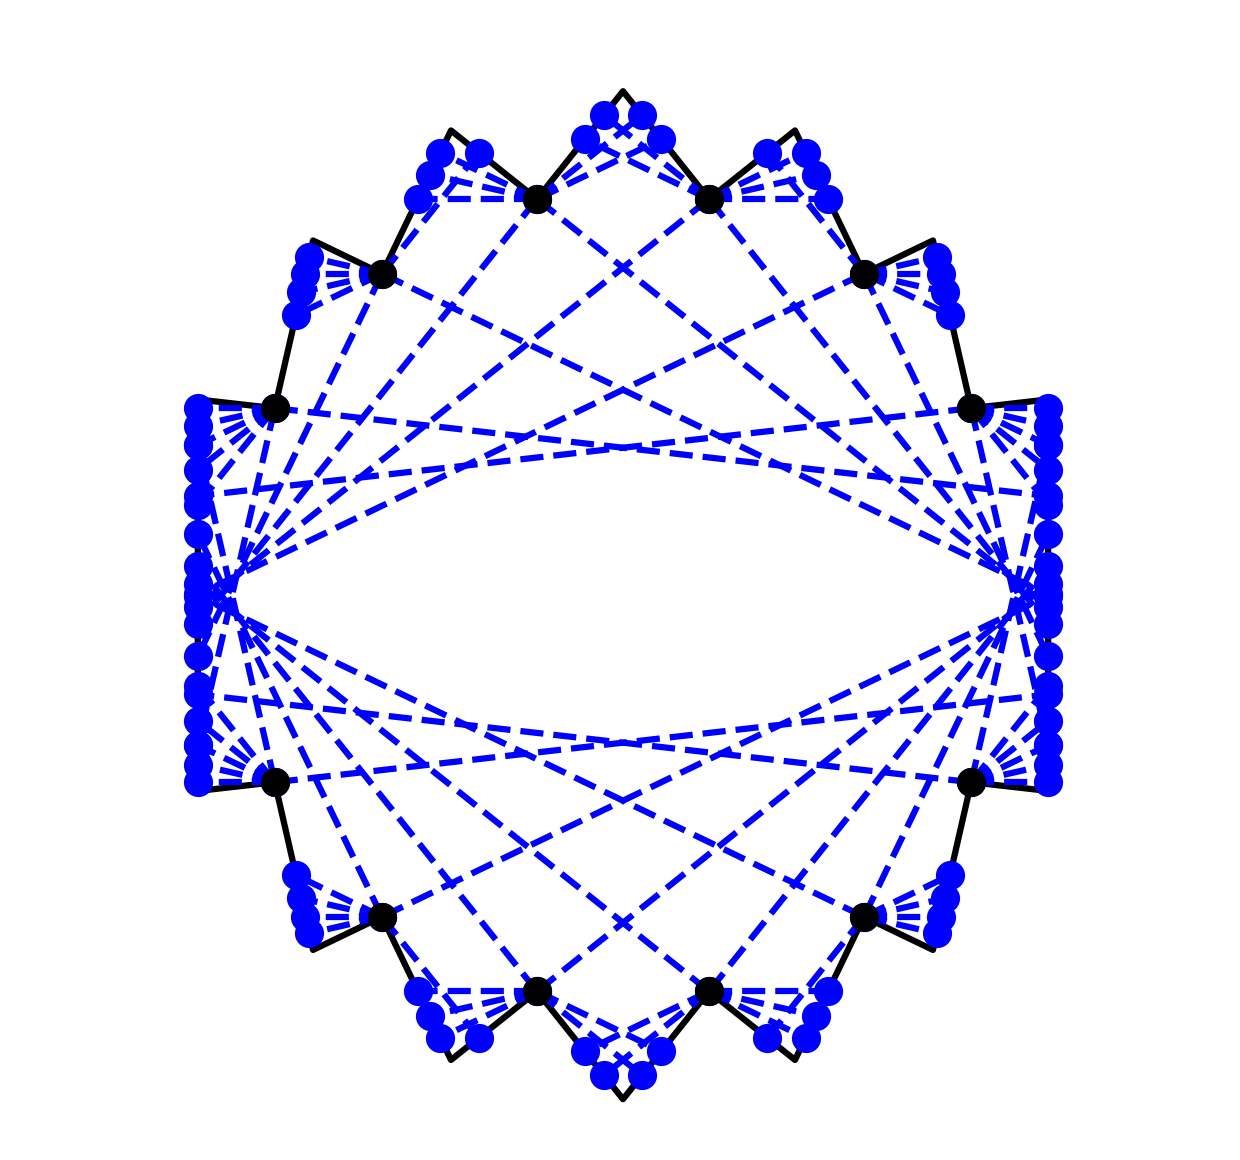
\includegraphics[width=0.7\linewidth]{images/chestnut_7.png}
}
\label{fig:t6}
}\\
\caption{The worse case polygon for $t = 4$ and $t = 6$}
\label{fig:chestnut}
\end{figure}

Let $n = 4t+2$, where $t$ is a positive integer. We design a polygon with $r = 2t$ reflex vertices. The polygon is symmetric with respect to its medium horizontal line. In the top half, the reflex vertices are uniformly located on a circle and thus they are visible to each other; the convex vertices are chosen so that they are outside the circle and the line through an edge will not intersect other edges. Each reflex vertices will have at least $t-1$ new vertices in its partial local sequence. All vertices in the top half can see each vertex in the bottom half and vice versa. So there will be $2t(t-1)+n$ vertices in the polygon after we insert all new vertices in the partial local sequence for all reflex vertices. Each of them can see at least $t(t-1)+n/2$ other vertices. The final complexity for the bounce visibility diagram is $\Theta ((2t(t-1)+n)(t(t-1)+n/2)) = \Theta (t^4) = \Theta(n^4)$. Fig~\ref{fig:chestnut} shows the polygons for $t = 4$ and $t=6$ with all the vertices in the partial local sequences.
% show the diagram to edge 
% show the fix bounce
% show the periodic behavior
% show the gap navigation
% show we could find equivalent class on theta
% \begin{itemize}
% \item Big O complexity of construction, and size of resulting graph


\section{BVD as an Information Space}

\subsection{Augmenting the Diagram with Dynamical Information}

\begin{itemize}
\item Laser Beams - laser beams form new, internal edges of the polygon. They can be added to the bounce visibility graph by marking all the edges which represent bounces that would cross the laser beam with a special symbol. different symbols for distinguishable beams. If beam is encountered, only propagate state estimate forward along edges with that symbol. To guarantee reduction in uncertainty, put laser beams in positions that break graph symmetry {\color{red} flesh out this idea}
\item Pebbles
\item Cameras
\end{itemize}

\section{Task Formulation}

We will now show how to formulate many common robot task specifications in terms
of the data structure described above. The discretization of the continuous
environment allows us to now reason over trajectories through a graph.


\subsection{Navigation}

Here, we define the \emph{navigation} task as:

Given an environment $P$, a start set of possible robot positions along the
environment boundary $S$, and a goal set $G$, determine a strategy $\pi$ which
will be guaranteed to take the robot from any point in $S$ to a point in $G$.

If the start set $S$ is such that it lies entirely within one of the equivalence
classes of the data structure, a navigation query is simple - the start set in
the graph is a single node, and the query is solved by a shortest path from this
node to the nodes representing the goal set. The shortest path will correspond
to the navigation strategy with the fewest number of bounces.

It may be
interesting to instead look to solve the navigation problem with different
criteria than the smallest number of bounces - for instance, we may look for a
strategy which uses the fewest number of bounce angles, or has the fewest number
of switches between bounce angles (especially useful for a robot which changes
its bounce angle mechanically).

If the start set $S$ lies in more than node of the graph, things get a bit
trickier.


Their approach can be replicated with the current work by the following
procedure: take the {\color{red}NAME} graph, and remove edges which represent unsafe actions.
Also need to add a corner finding strategy (how do we know when we've found the
corner?). 

\subsection{Patrolling}

In prior work {\color{red} cite}, it was shown that stable limit cycles exist for fixed bouncing in regular polygons, for some ranges of bounce angles. These results also hold for convex polygons in general.

- sketch main idea: contraction mapping from one edge back to itself -> fixed point on edge -> limit cycle

What about nonconvex polygons?

- easy case: choose subset of edges that, if extended to their intersections, form convex polyon

- harder case: choose periodic sequence of sequentially visible edges

- trickiness of composing functions: range of angles which lead to limit cycle must be supported by every range/domain along compositional chain

- complexity of this search: all cycles in graph?

\subsection{Localization}

incorporate "Localization with Limited Sensing"



\section{Toward a Hierarchy of Bouncing Robots}




\section{Open Questions and Future Work}

randomized plans?

\section{Conclusion}



\bibliographystyle{IEEEtran}
\bibliography{refs}

\end{document}
